\documentclass[a4paper, 12pt]{ctexart}

\usepackage{enumerate}
\usepackage{graphicx}
\usepackage{listings}
\usepackage{xcolor}
%\usepackage{fancyhdr}


% code listings
\lstdefinestyle{customc}{
	belowcaptionskip=1\baselineskip,
	breaklines=true,
	frame=L,
	xleftmargin=\parindent,
	language=C,
	showstringspaces=false,
	basicstyle=\footnotesize\ttfamily,
	keywordstyle=\bfseries\color{green!40!black},
	commentstyle=\itshape\color{purple!40!black},
	identifierstyle=\color{blue},
	stringstyle=\color{orange},
}

\lstset{basicstyle=\ttfamily\color{brown},
	showstringspaces=false,
	commentstyle=\color{red},
	keywordstyle=\color{blue}
}

%%%%%%%%%%%% author  %%%%%%%%%%%%%%%%
\author{金国栋\\
	\and
	韩涵\\
	\and
	黄文韬\\
	\and
	陈成\\
}
\title{分布与并行数据库Pard系统实验报告}
\date{\today}


%%%%%%%%%%%%%%%==============  \begin{document}  ====================%%%%%%%%%%%%%%%%%%%
\begin{document}

\maketitle%
\hspace{8em}
\begin{figure}[h]
	\centering
	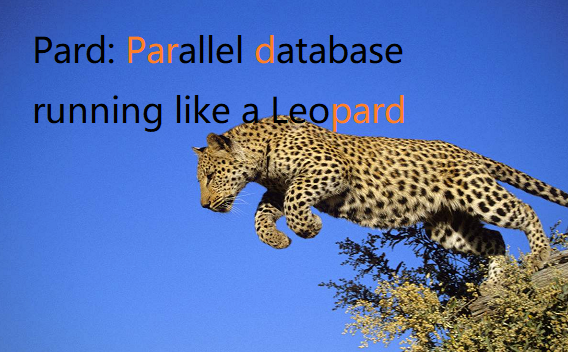
\includegraphics[width=0.7\linewidth]{figure/leopard.png}
\end{figure}




\newpage
 
\tableofcontents
 
 
\section{系统概述}
\subsection{任务回顾}
我们要实现一个分布式数据库系统,即通过网络将多个不同的局部数据库系统连接起
来,使得用户可以通过分布式数据库管理系统达到透明性管理的目的。
在我们具体的实例中,我们通过网络将 3 个不同站点的4个局部数据库连接起来,并可以通
过分布式数据库管理系统(Client)进行数据库创建,数据分片、分配、导入及 SQL 操作等
管理,支持水平划分、垂直划分。


\subsection{运行环境}
Java8 以上,postGRESQL,Linux操作系统。

\subsection{开发环境}
Git + Intellij IDEA + Java8 + Maven3.3.9+

 
 Compilation Without Running Unit Tests:
 
\lstinline[language=bash]|mvn clean package -DskipTests|

\lstinline|mvn clean compile -DskipTests|
 
 Compilation With Running Unit Tests:
 
\lstinline|mvn clean package or mvn clean compile|
 
\begin{lstlisting}

\end{lstlisting}
 
 Tips:
\begin{enumerate}[1]
 	\item Compile locally to ensure everything is ok before pushing to Github.
 	\item Pay attention to CheckStyle. Make sure your code style satisfies the code style rules.
 \end{enumerate}
 
 
 
\section{总体设计}
Pard整体运行概念如图\ref{fig:archi},用户通过命令行与某个主节点Pard Node上的client进行交互,
总共有三个场地,分别命名为 site1 、site2 、site3,四个postgresql作为Slave DB。
理论上来讲这样其实是有点怪异,某些优化技术是需要和本地数据库做深度定制和交互的,但是本门课程是分布与并行数据库,重在分布与并行的优化技术,
没有太多精力再做一个深度定制的本地数据库。

\begin{figure}[htbp]
	\centering
	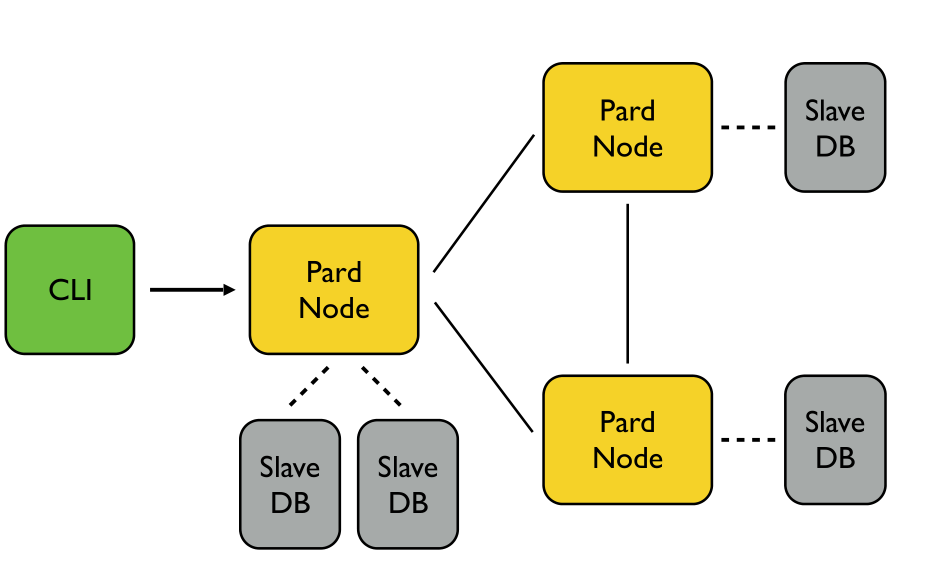
\includegraphics[width=\linewidth]{figure/architecture.png}
	\caption{Pard整体运行概念图}
	\label{fig:archi}
\end{figure}

Pard单个节点的架构如图\ref{fig:node1}。每个节点都有可能成为与用户直接交互的节点,应用层面诸如Client、Web UI
是用户可见的抽象层级。下面来看底层实现。Pard收到用户输入的SQL语句,先做SQL的语法解析,拿到抽象语法树AST。
依据数据在不同站点的划分,数据本身的分布特性,对AST做优化改造。Job Planner生成物理的查询执行计划,
Job scheduler发送给各个节点
去做具体的任务执行,安排好job执行的顺序、同步异步等等,使用一定的并行加速技术。
各个节点还有存储管理模块,负责管理数据在内存中的组织形式(column-store, buffer management, 数据压缩等等)。
通讯模块具体分两类:一类是任务的通信,使用RPC技术发送较小数据量的任务通知;
另一类是SQL执行需要的大批量数据的通信,我们使用Netty做大批量数据的异步传输。
Catalog使用etcd进行分布式存储,etcd遵循的raft协议可以确保各个节点GDD的一致性。
Executor是本地执行器,Connetor连接pard到本地的postGRESQL。

\begin{figure}[htbp]
	\centering
	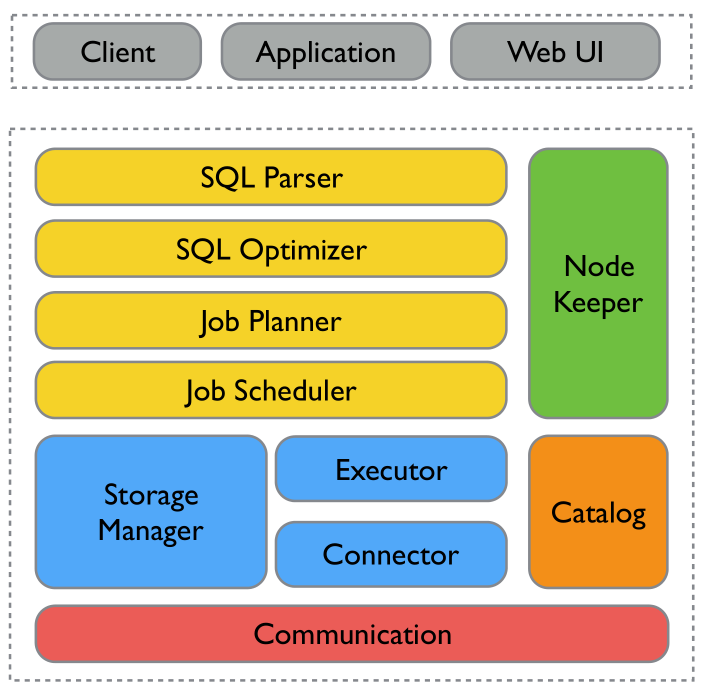
\includegraphics[width=0.7\linewidth]{figure/pard-node-in.png}
	\caption{Pard单个节点的架构}
	\label{fig:node1}
\end{figure}


\subsection{时间安排}
如图\ref{fig:tl}。

\begin{figure}[htbp]
	\centering
	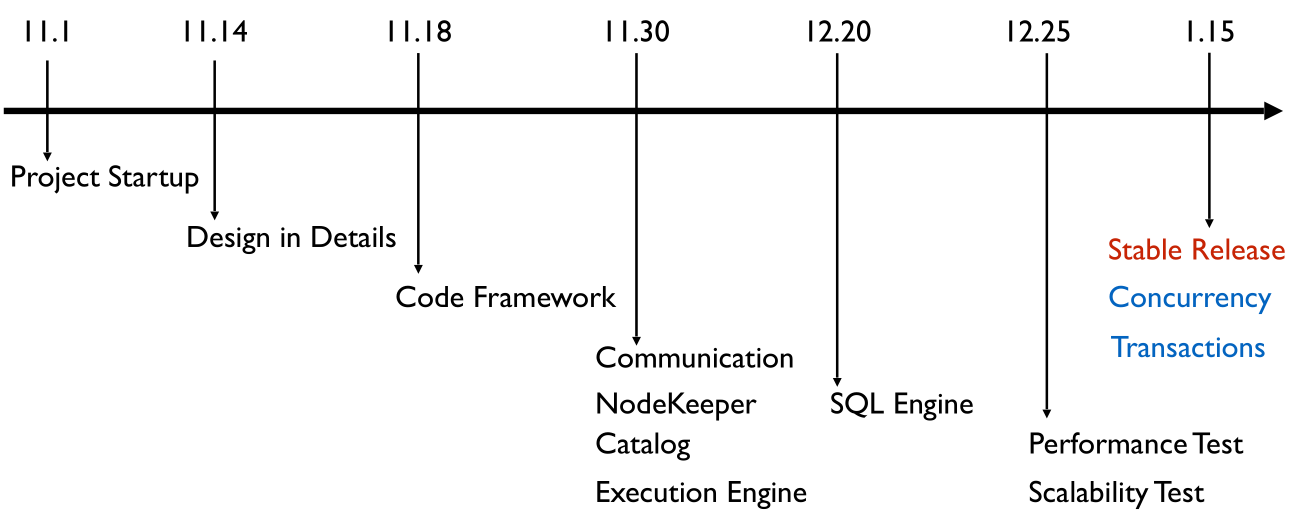
\includegraphics[width=\linewidth]{figure/timeline.png}
	\caption{时间安排timeline}
	\label{fig:tl}
\end{figure}
在国栋师兄的英明领导下,我们pard小组稳中有进,时间安排还算合理。

\section{各模块详细设计}

\subsection{SQL Engine}
\subsection{Execution Engine}


\subsection{Communication}


\subsection{Catalog}

\subsection{Project Dependency Management}

\section{任务分工及小结}

\subsection{金国栋的小结}

\subsection{韩涵的小结}

\subsection{黄文韬的小结}

\subsection{陈成的小结}





 
\end{document}